\documentclass{article} 
\usepackage[utf8]{inputenc} 
\usepackage{graphicx}
\newcommand{\figautorefname}{figure}
\newcommand{\secautorefname}{section}
\newcommand{\subsecautorefname}{subsection}
\newcommand{\subsubsecautorefname}{subsubsection}

\title{Biometric Authentication System Documentation} \author{Authors}
\date{\today}

\begin{document}

\maketitle

\section{Introduction} The Biometric Authentication System is a prove of concept of an IoT
solution designed to provide security authentication through biometric verification, including
galvanic skin response, heart rate analysis, and facial recognition. This
project's primary objective is to establish a user-friendly system
for authenticating individuals in secure environments as well as experimenting and learning with IoT devices. The following
documentation comprises detailed descriptions of system components,project milestones, a user story depicting the system's functionality, and
technical insights into the component integration and operation.

\section{General Project Milestones} The development of the Biometric
Authentication System was achieved through the accomplishment of several key
milestones. These milestones collectively ensured the project's progress was
systematically tracked and adhered to the proposed timeline. Note that component specific milestones with more
detailed information, priorities and dependencies can be found on \autoref{component-implementations}

\begin{enumerate} 
    \item \textbf{Project Initiation:} Defining scope, objectives,
and resource allocation. 
\item \textbf{Component Sourcing and Assembly:} Hardware setup of the development environment. 
\item \textbf{System Design:} Architecting overall system interactions and data flow.
\item \textbf{Component Integration:} Ensuring seamless operation between
different system modules. 
\item \textbf{Software Development:} Writing and
testing code for individual components and overall system coordination. 
\item \textbf{Project Wrap-Up:} Final evaluation, documentation,
and project delivery. 
\end{enumerate}

\section{Component Implementations}\label{sec:component-implementations} This section outlines the individual
components that comprise our system, detailing their objectives, functionalities,
and integration with the broader system context.

\subsection{RaspberryPi}

\subsubsection{Objective and Functionality}
The RaspberryPi is the backbone of the project, it serves as the MQTT broker and merges the collected data from both the Biometric Sensors and the camera it has attached to provide a prediction of who may the user interacting with system be, sending that final prediction to the Monitor System. Its responsibilites include:
\begin{itemize}
    \item Subscribing to and processing biometric data from the ESP-01 module attached to biometric sensors via MQTT.
    \item Processing data from the webcam connected to the RaspberryPi via usb and running it through a neural network to get a prediction of who is the user in the picture.
    \item Run the biometric data obtained through MQTT and the result of the neural network through a decision tree to get a final prediction of who is the user interacting with the system.
    \item Sending the final result to the 'rpi/prediction' topic so the System Monitor can show the result.
\end{itemize}

\subsubsection{Project Definition and Milestones}
The development of the RaspberryPi system involved the following milestones:
\begin{enumerate}
    \item Setting up an MQTT broker to handle all the IoT devices communications.
    \item Establishing MQTT communication to receive biometric data and send predictions.
    \item Training a neural network to work with the webcam input and predict which user is in front of it.
    \item Training a classification tree to get a final prediction using both biometric data and neural network prediction.
\end{enumerate}

\subsubsection{Achieved milestones, execution order, priority, and dependencies}
\begin{enumerate}
    \item \textbf{Milestone 1: Setting up an MQTT broker}
        \begin{enumerate}
            \item \textit{Priority:} High. Fundamental for all the data transmission.
            \item \textit{Dependencies:} Basic WiFi setup.
            \item \textit{Execution Order:} First, as it is crucial for data reception.
            \item \textit{Assigned to:} Pablo
        \end{enumerate}

    \item \textbf{Milestone 2: Establishing MQTT communication to receive and send data}
        \begin{enumerate}
            \item \textit{Priority:} Medium. Important for working with real data.
            \item \textit{Dependencies:} Successful MQTT setup.
            \item \textit{Execution Order:} Second, building upon established communication.
            \item \textit{Assigned to:} Pablo
        \end{enumerate}

    \item \textbf{Milestone 3: Training neural network}
        \begin{enumerate}
            \item \textit{Priority:} High. Essential for effective prediction.
            \item \textit{Dependencies:} Functional hardware setup (webcam).
            \item \textit{Execution Order:} Third, getting a first prediction.
            \item \textit{Assigned to:} Ferran
        \end{enumerate}

    \item \textbf{Milestone 4: Training a classification tree}
        \begin{enumerate}
            \item \textit{Priority:} Medium. Important for a more accurate prediction.
            \item \textit{Dependencies:} Functioning MQTT communication and neural network.
            \item \textit{Execution Order:} Fourth, finalizing the machine learning prediction.
            \item \textit{Assigned to:} Ferran
        \end{enumerate}

    \item \textbf{Milestone 5: Sending the results}
        \begin{enumerate}
            \item \textit{Priority:} High. Essential for system effectiveness.
            \item \textit{Dependencies:} Functioning MQTT communication and classification tree.
            \item \textit{Execution Order:} Fourth, last step towards getting a prediction shown to the user.
            \item \textit{Assigned to:} Oriol
        \end{enumerate}
\end{enumerate}

\subsubsection{Hardware setup}
The hardware setup for the RaspberryPi comprises:
\begin{itemize}
    \item A RaspberryPi 4 with WiFi capabilites.
    \item A logitech webcam with usb connection.
\end{itemize}

\subsubsection{Software Implementation}
The software, written in python has the key functions:
\begin{itemize}
    \item Recieving biometric data from 'sensor3/galvanic' and 'sensor3/heart' topics.
    \item Triggering a neural network prediction through the webcam obtained footage.
    \item Run the result from the neural network and the biometric data through a classification tree.
    \item Publish the final prediction to the 'rpi/prediction' topic.
\end{itemize}
The operating system (RaspberriPi OS Lite) is responsible of connecting to WiFi and running MQTT broker. So basically it has to:
\begin{itemize}
    \item Run a service for MQTT broker that launches on startup.
    \item Establish WiFi connection.
    \item Run a service that initializes the prediction pipeline when a user is detected.
\end{itemize}

\textbf{\textit{NOTE}}: The data collection for training the classification tree has also been done on the RaspberryPi as well as the training itself, code for replicating this steps can be found on the project repository.

\subsubsection{Testing}
Testing has been mainly focused on the machine learning aspect, since getting accurate results was non trivial. By generating artificial data (data augmentation) it was possible to finally achieve a more convincing accuracy. Regarding MQTT, setting up the broker was a very straight forward process with no trouble.

\subsubsection{Dedication Time}
Approximately 30 hours were dedicated to developing the RaspberryPi system, using most of the time on the machine learning aspect.

\subsubsection{Challenges and Solutions}
\begin{itemize}
    \item \textbf{Hardware Challenges:} Collecting footage from the usb webcam.
    \item \textbf{Software Challenges:} Getting an accurate prediction from the model. Using a foundational model trained for object detection wasn't working very well for telling faces apart so the solution provided is to use a representative item for each member of the group which is what is placed in front of the camera, this way the neural network can tell us apart easily.
\end{itemize}

\subsubsection{Hardware and Software Integration}
The only hardware used on this setup was a webcam connected through usb to the RaspberryPi.

\subsubsection{MQTT Topics}
\begin{itemize}
    \item \textbf{sensor3/heart:} This is the topic used to collect heart rate biometric data.
    \item \textbf{sensor3/galvanic:} Provides galvanic resistance data, and together with the first topic, this two provide the full biometric data needed.
    \item \textbf{rpi/prediction:} Topic used to publish the result of the prediction.
\end{itemize}

\subsubsection{Conclusion}
The development on the RaspberryPi system was a very interesting experience, it was the first time working with machine learning for some of us and it was very challenging to get an accurate prediction, but after some research and testing it was possible to get a good result. The MQTT broker setup was very straight forward and it was easy to get it working.

\subsection{System Monitor}

\subsubsection{Objective and Functionality}
The System Monitor is a pivotal component in a biometric data-based framework for user access and verification. It serves two main functions: position detection using user location data and user identification. The System Monitor's functionalities include:
\begin{itemize}
    \item Subscribing to and processing location data from two ESP-01 modules with ultrasonic sensors via MQTT.
    \item Displaying user location and verification data on an LCD screen.
    \item Visually representing user proximity using an LED bar.
\end{itemize}

\subsubsection{Project Definition and Milestones}
The development of the System Monitor involved the following milestones:
\begin{enumerate}
    \item Establishing MQTT communication to receive data from ultrasonic sensors.
    \item Integrating and configuring the LED bar and LCD with the ESP32.
    \item Developing and testing the software for proximity detection and data display.
    \item Efficient multitasking and task synchronization within FreeRTOS.
\end{enumerate}

\subsubsection{Achieved milestones, execution order, priority, and dependencies}
\begin{enumerate}
    \item \textbf{Milestone 1: Establishing MQTT Communication}
       - \textit{Priority:} High. Fundamental for data transmission.
       - \textit{Dependencies:} Basic WiFi setup.
       - \textit{Execution Order:} First, as it is crucial for data reception.

    \item \textbf{Milestone 2: LED Bar and LCD Integration}
       - \textit{Priority:} Medium. Important for user interface.
       - \textit{Dependencies:} Successful MQTT setup.
       - \textit{Execution Order:} Second, building upon established communication.

    \item \textbf{Milestone 3: Software Development}
       - \textit{Priority:} High. Essential for functionality.
       - \textit{Dependencies:} Functional hardware setup.
       - \textit{Execution Order:} Third, focusing on processing and display.

    \item \textbf{Milestone 4: Multitasking and Task Synchronization}
       - \textit{Priority:} High. Critical for system reliability.
       - \textit{Dependencies:} Completion of initial software development.
       - \textit{Execution Order:} Fourth, finalizing the system integration.
\end{enumerate}

\subsubsection{Hardware Development}
The hardware setup for the System Monitor comprises:
\begin{itemize}
    \item An ESP32 microcontroller connected to a breadboard.
    \item An LED bar and an LCD screen interfaced with the ESP32 for display.
    \item Two ESP-01 modules, each with an ultrasonic sensor, for distance measurement.
\end{itemize}

\subsubsection{Software Implementation}
The software, written in C++, leverages FreeRTOS for effective multitasking. Key functions include:
\begin{itemize}
    \item \texttt{WiFiTask} for managing WiFi connectivity.
    \item \texttt{MQTTTask} for handling MQTT communication.
    \item \texttt{LCDDisplayTask} and \texttt{checkForPresenceAndDirection} for controlling the display based on sensor data.
    \item Semaphore (\texttt{xSemaphoreLCD}) to ensure safe LCD access.
\end{itemize}

\subsubsection{Interaction with Other Components}
The System Monitor interacts with the ESP-01 modules to determine the user's location based on distance data, which is then displayed on the LED bar and LCD screen.

\subsubsection{Testing}
Testing ensured accurate sensor data transmission via MQTT and responsive displays on the LED bar and LCD. An iterative approach was applied to refine the system's performance.

\subsubsection{Dedication Time}
Approximately 20 hours were dedicated to developing the System Monitor, focusing on both hardware assembly and software programming.

\subsubsection{User Story}
As a user approaches, the System Monitor detects their presence, lighting up the LED bar and displaying their approximate location (left, right, or center) on the LCD screen, providing real-time feedback.

\subsubsection{Challenges and Solutions}
\begin{itemize}
    \item \textbf{Hardware Challenges:} Complex wiring and space constraints on the breadboard, along with troubleshooting LED issues.
    \item \textbf{Software Challenges:} Establishing reliable communication and processing sensor data accurately. Achieved through careful coding and testing.
\end{itemize}

\subsubsection{Hardware and Software Integration}
\begin{figure}[ht]
    \centering
    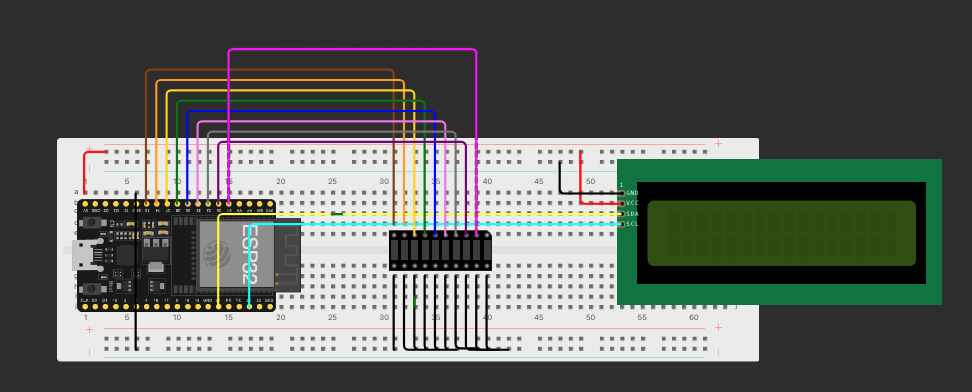
\includegraphics[width=0.8\textwidth]{../images/activity_monitor_scheme.png}
    \caption{ESP32 with LED bar and LCD display connected on a breadboard.}
    \label{fig:esp32_system_monitor}
\end{figure}

\subsubsection{Microcontroller Interaction Protocol}
The System Monitor project involves coordinated communication between multiple microcontrollers, primarily the ESP32 and two ESP-01 modules. The communication is structured as follows:

\paragraph{Communication Protocol}
The project utilizes the MQTT (Message Queuing Telemetry Transport) protocol, a lightweight and efficient messaging protocol ideal for IoT applications. This protocol is chosen for its low bandwidth usage and its ability to provide reliable communication over WiFi.

\paragraph{WiFi Configuration}
Each microcontroller in the system is configured to connect to a WiFi network, enabling them to send and receive data over the network. The network credentials (SSID and password) are programmed into the microcontrollers.

\paragraph{Data Flow and Configuration}
The ESP-01 modules, each equipped with an ultrasonic sensor, collect distance data and publish this information to specific MQTT topics. The ESP32, acting as the central unit, subscribes to these topics to receive the data.

\subsubsection{MQTT Tree Structure}
The MQTT protocol in the System Monitor project uses a structured approach to manage the data flow. Below is the outline of the MQTT topics and their functions:

\paragraph{MQTT Topics}
\begin{itemize}
    \item \textbf{sensor1/distance:} This topic is used by the first ESP-01 module. It publishes the distance data measured by its connected ultrasonic sensor. The ESP32 subscribes to this topic to receive updates on the user's distance from this sensor.
    \item \textbf{sensor2/distance:} Similar to the first, this topic is for the second ESP-01 module. It provides distance data from its sensor, allowing the ESP32 to determine the user's location relative to this second sensor.
\end{itemize}

\paragraph{Data Organization and Utilization}
The data sent to these topics include numerical values representing the measured distances. The ESP32, upon receiving this data, processes it to determine the user's proximity and location. Based on these calculations, the ESP32 then controls the LED bar and the LCD display to provide real-time feedback about the user's position.
\documentclass{article}
\usepackage[utf8]{inputenc}
\usepackage{graphicx}

\begin{document}

\section{Integration of Biometric Sensors with Arduino NANO-BLE33 and ESP-01}

\subsection{Objective and Functionality}
The user data collector is the part of the system responsible of collecting the users heart rate and galvanic skin resistance in order to later predict who is that user.
\begin{itemize}
    \item Reading BPM and galvanic resistance data from the sensors on the Arduino NANO
    \item Getting the collected data from the Arduino to the ESP01 module through serial.
    \item Publishing the collected data to the corresponding MQTT topics (sensor3/heart and sensor3/galvanic)
\end{itemize}

\subsection{Project Definition and Milestones}
The development of the user data collector involved the following milestones:
\begin{enumerate}
    \item Read data from BPM.
    \item Read data from galvanic.
    \item Get data from Arduino to ESP01.
    \item Establishing connection with MQTT.
    \item Publish the results on their corresponding topics.
\end{enumerate}

\subsection{Achieved milestones, execution order, priority, and dependencies}
\begin{enumerate}
    \item \textbf{Milestone 1: Read data from BPM and galvanic}
       - \textit{Priority:} High. Fundamental for data collection.
       - \textit{Dependencies:} Working hardware setup.
       - \textit{Execution Order:} First, as it is the backbone of this system.

    \item \textbf{Milestone 2: Establish connection with MQTT and publish data}
       - \textit{Priority:} Medium. Important, the rest of the system needs this data.
       - \textit{Dependencies:} Working WiFi setup.
       - \textit{Execution Order:} Second, needed for debugging the data retrieval from Arduino to ESP01.

    \item \textbf{Milestone 3: Getting data from Arduino to ESP01}
       - \textit{Priority:} High. Essential for usage of real data.
       - \textit{Dependencies:} Functional hardware setup and MQTT communication.
       - \textit{Execution Order:} Third, focusing on data transmission.
\end{enumerate}

\subsection{Hardware setup}
The biometric data collection system comprises the following hardware components:
\begin{itemize}
    \item \textbf{Arduino NANO-BLE33:} Central to the collection and initial processing of biometric data, including heart rate and galvanic skin response (GSR).
    \item \textbf{ESP-01:} Functions as a WiFi module, enabling the Arduino NANO-BLE33 to connect to the internet and transmit data using MQTT.
    \item \textbf{MAX30105 Heart Rate Sensor:} Connected to the Arduino for monitoring the user's heart rate.
    \item \textbf{GSR Sensor:} Attached to the Arduino for measuring galvanic skin response.
\end{itemize}

\subsection{Hardware setup diagram}
The following diagram illustrates the physical connections between the Arduino NANO-BLE33, ESP-01, and the biometric sensors (Heart-rate and GSR sensors).

\begin{figure}[h]
    \centering
    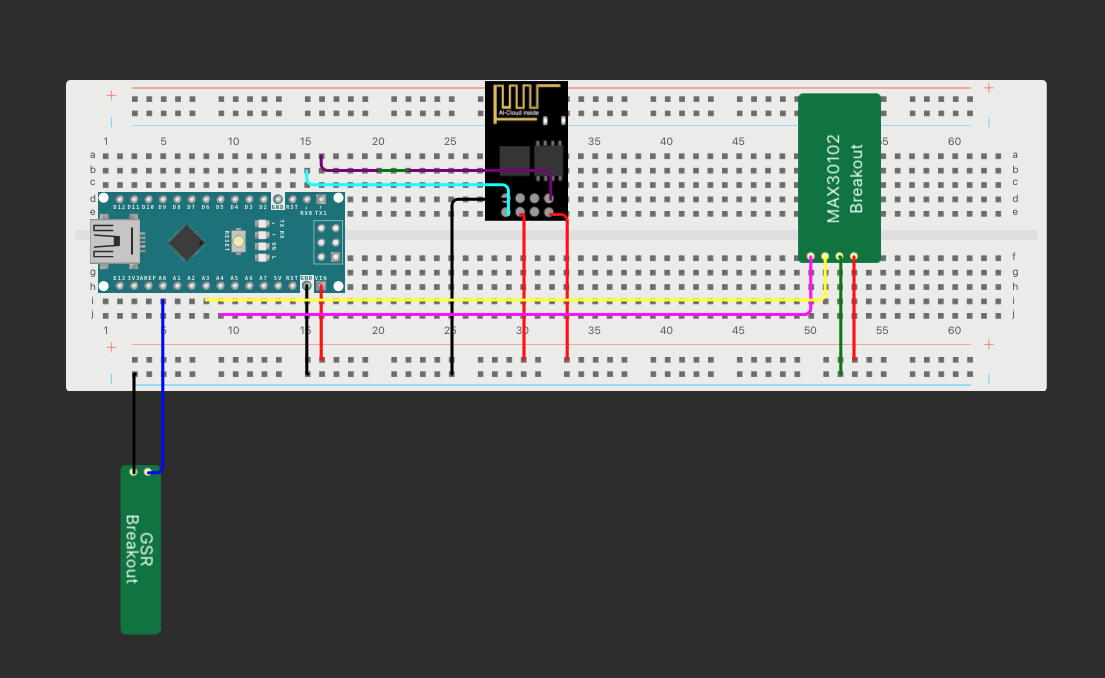
\includegraphics[width=0.8\textwidth]{../images/gsr&heart.png}
    \caption{Hardware connection diagram of Arduino NANO-BLE33 with ESP-01 and biometric sensors.}
    \label{fig:hardware-setup}
\end{figure}


\subsection{ESP-01}
The ESP-01 module is programmed to receive the biometric data from the Arduino NANO-BLE33 and publish it to an MQTT broker. The implementation covers:
\begin{itemize}
    \item Establishing a WiFi connection.
    \item Setting up MQTT client and handling reconnections.
    \item Reading data from the Arduino via Serial communication.
    \item Publishing the received data to the MQTT broker under the topic "sensor3/data".
\end{itemize}

\subsection{Challenges and Solutions}
During the integration of the biometric sensors with the Arduino and ESP-01, several challenges were encountered and subsequently addressed:
\begin{itemize}
\item \textbf{Serial Communication:} The initial challenge was to establish a stable and reliable serial communication between the Arduino NANO-BLE33 and the ESP-01. This was achieved by setting a consistent baud rate and implementing a protocol to ensure complete data packets were sent and received.
\item \textbf{MQTT Connectivity:} Maintaining a stable MQTT connection, especially handling reconnections and network instability, was critical. This was addressed by implementing a reconnection strategy in the ESP-01’s software.
\end{itemize}

\subsection{Dedication Time}
Approximately 30 hours were dedicated to developing the user data collection system, using most of the time on playing with malfunctioning or hard to use sensors.

\subsection{MQTT Topics}
\begin{itemize}
    \item \textbf{sensor3/heart:} This is the topic used to publish heart rate biometric data.
    \item \textbf{sensor3/galvanic:} Used to publish galvanic resistance data.
\end{itemize}

\subsection{Conclusion}
The integration of the Arduino NANO-BLE33 with the ESP-01 for biometric data collection and transmission via MQTT represents a significant advancement in the biometric verification system. This setup not only provides real-time data monitoring but also enhances the system's capability to make a prediction on the user's identity.

\end{document}

\documentclass{article}
\usepackage[utf8]{inputenc}
\usepackage{graphicx}

\begin{document}

\section{Presence and location}

\subsection{Objective and Functionality}
The presence and location is a set of two devices each with an ultrasonic sensor that determine user presence and location (left-right). Each of the sensors is responsible of sending collected data to their respective topic (sensor1/distance or sensor2/distance).

\subsection{Project Definition and Milestones}
The development of the presence and location system just involves establishing an MQTT connection with the broker to send the collected data from the ultrasonic sensors.

\subsection{Achieved milestones, execution order, priority, and dependencies}
\begin{enumerate}
    \item \textbf{Milestone 1: Establishing MQTT Communication}
       - \textit{Priority:} High. Fundamental for data transmission.
       - \textit{Dependencies:} Basic WiFi setup.
       - \textit{Execution Order:} First, as it is crucial for data reception.

    \item \textbf{Milestone 2: Send the collected that from the sensor}
       - \textit{Priority:} High. Essential for functionallity
       - \textit{Dependencies:} Successful MQTT setup.
       - \textit{Execution Order:} Second, building upon established communication.
\end{enumerate}

\subsection{Hardware setup}
The hardware setup for the location and presence comprises:
\begin{itemize}
    \item Two ESP-01 modules.
    \item Two ultrasonic sensor, one for each ESP-01 module.
\end{itemize}

\subsection{Software Implementation}
The software, written in arduino programming language, has the following key functionalities:
\begin{itemize}
    \item Connect to WiFi (and try to reconnect if needed).
    \item Establish MQTT connection.
    \item Measure and calculate distance using ultrasonic sensor pins.
    \item Send the resulting data to the corresponding topic (sensor1/distance or sensor2/distance)
\end{itemize}

\subsection{Dedication Time}
Approximately 15 hours were dedicated to developing the System Monitor, mainly spent on finding out sensor malfunctioning given that the software implementation was simple and straightforward.

\subsection{Challenges and Solutions}
\begin{itemize}
    \item \textbf{Hardware Challenges:} Malfunctioning sensors which drove us crazy.
    \item \textbf{Software Challenges:} Processing sensor data accurately, since this cheap sensors can provide really confusing data.
\end{itemize}

\subsection{Hardware diagram}
\begin{figure}[ht]
    \centering
    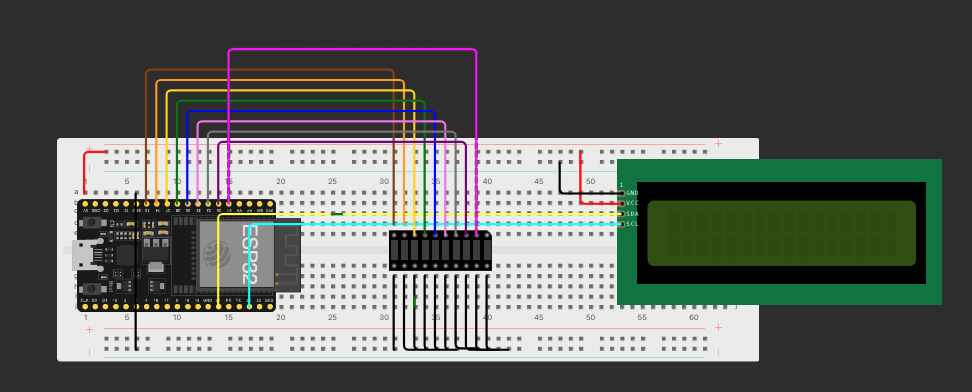
\includegraphics[width=0.8\textwidth]{../images/activity_monitor_scheme.png}
    \caption{Ultrasonic sensors connected to ESP01 modules.}
    \label{fig:esp32_system_monitor}
\end{figure}

\subsubsection{Data Flow and Configuration}

\subsection{MQTT Tree Structure}
The MQTT protocol in the presence and location project uses a structured approach to manage the data flow. Below is the outline of the MQTT topics and their functions:

\subsubsection{MQTT Topics}
\begin{itemize}
    \item \textbf{sensor1/distance:} This topic is used by the first ESP-01 module. It publishes the distance data measured by its connected ultrasonic sensor.
    \item \textbf{sensor2/distance:} Similar to the first, this topic is for the second ESP-01 module.
\end{itemize}

\subsubsection{Data Organization and Utilization}
The data sent to these topics include numerical values representing the measured distances. 

\end{document}


\section{User Story} As the user approaches the authentication system, he is
immediately detected by the ultrasonic sensors, which guide him to stand in the
optimal position for scanning. As he places his fingers on the biometric sensors,
his heart rate and skin resistance data are quietly collected and sent to the
Raspberry Pi. At the same moment, the user looks at the camera, and his facial
features are analyzed. The Raspberry Pi processes this information using
a neural network and merges the results of the facial prediction with the biometrics sensors
data by running them into a decision tree which outputs a final prediction, which appears on the screen
and will tell which of the authorized users matches with if any. Within seconds, if the system identifies the user, 
his name is displayed on the monitors.

\section{Final Project Conclusions} The development of the Biometric
Authentication System has been a path characterized by learning, adaptability,
and fighting with malfunctioning sensors. One of the main challenges was synchronizing data from various
biometric sensors with the real-time processing on the Raspberry Pi.
By applying concurrency principles we managed to overcome this challenges and end up with a significantly accurate system.

Overall, the system has realized robust biometric authentication with an
impressive accuracy rate. The modularity of the system design also allows for
easy updates and scalability.

For future work, we suggest exploring alternative biometric modalities such as
iris recognition or palm-print scanning to further enhance system security.
Additionally, implementing machine learning models with more extensive datasets
can offer continued improvement in recognition accuracy and pave the way for
personalized user experiences.

\section{Technical Documentation}
For a in depth technical documentation of the system, detailed 
instructions on how to setup the system and how to use it, please refer to the following specifications
(which can also be found in the project repository):

\subsection{Raspberry Pi 4 Configuration}\label{raspberry-pi-4-configuration}

We use the raspberry pi 4 as a: - MQTT Broker - EdgeImpulse node for
running the IA for detecting objects.

\subsubsection{Configure the raspberry pi}\label{configure-the-raspberry-pi}

You can configure your raspberry pi liunx image with
\href{https://github.com/raspberrypi/rpi-imager}{rpi imager}, which
comes pretty handy since you can:

\begin{itemize}
\item
  Enable wifi with an SSID and password.
\item
  Enable ssh and give it a public key that is allowed to connect to the
  rpi
\item
  Add a username and password
\end{itemize}

This saved us a lot of time, and we didn't have to use any ethernet
cable or screen for configuring it.

\subsubsection{Install mosquitto broker}\label{install-mosquitto-broker}

Install mosquitto with:

\begin{verbatim}
# We're using the raspbian lite image for the rpi
$ sudo apt-get update && sudo apt-get upgrade
$ sudo apt-get install mosquitto
\end{verbatim}

\subsubsection{Run mosquitto broker}\label{run-mosquitto-broker}

Once mosquitto is installed, copy our configuration file and run it
with:

\begin{verbatim}
$ mosquitto -c mosquitto.conf -v
\end{verbatim}

It will serve the mqtt server on port 1883.

\subsubsection{}\label{section}

\subsection{Configure your Linux Computer as an AP of the
project}\label{configure-your-linux-computer-as-an-ap-of-the-project}

Please watch the figure on assets/network-diagram.png for understanding
this article.

\subsubsection{Hardware you need:}\label{hardware-you-need}

\begin{itemize}
\tightlist
\item
  A wifi adapter network that supports AP virtual interface (we used an
  Alfa AWUS036ACH-C, but some integrated wifi cards can handle
  promiscuous mode and AP virtual interfaces)
\item
  A computer running Linux with systemd.
\end{itemize}

\subsubsection{Software you need:}\label{software-you-need}

\begin{itemize}
\tightlist
\item
  \href{https://github.com/lakinduakash/linux-wifi-hotspot}{Linux Wifi
  Hotspot}
\end{itemize}

\subsubsection{Brief overview of the
steps:}\label{brief-overview-of-the-steps}

\begin{itemize}
\tightlist
\item
  Patch the create\_ap program that comes with Linux Wifi Hotspot for
  enabling an static IP for the raspberry pi.
\item
  Change the Internet interface and the Wifi interface on the ap.conf.
\item
  Execute!
\end{itemize}

\paragraph{Patch the create\_ap
program}\label{patch-the-create_ap-program}

By default,
\href{https://github.com/lakinduakash/linux-wifi-hotspot}{Linux Wifi
Hotspot} executes: -
\href{https://wiki.gentoo.org/wiki/Hostapd}{hostapd}: For creating the
wifi access point -
\href{https://wiki.archlinux.org/title/Dnsmasq}{dnsmasq}: For adding
DHCP server to the network. -
\href{https://wiki.archlinux.org/title/Iptables}{iptables}: For
forwarding all the traffic that comes from the AP network (in other
words, in your AP network your computer acts as a router, forwarding the
packets).

Using the \textbf{create\_ap} script that comes with the Linux Wifi
Hotspot packages become very handy, since we don't have to create the
hostapd, dnsmasq and iptables ourselves, buuut has a catch: \textbf{it
doesn't allow us to put dhcp rules (such as static ip for the raspberry
pi) on his config file}.

This is because the \textbf{create\_ap} script automatically generates
the configuration for hostapd, dnsmasq and iptables given the
configuration file you gave it (and obviously this config file doesn't
have an option for adding dhcp rules\ldots),
\href{https://github.com/lakinduakash/linux-wifi-hotspot/blob/d73242ab812284b5ed65275f630b8bc306b725c5/src/scripts/create_ap\#L1762}{you
can watch the code that generetes the dnsmasq rules here}.

So, we had to patch the \textbf{create\_ap} script for adding our custom
rule! Yay! First of all find where is the \textbf{create\_ap} script
living on your computer:

\begin{Shaded}
\begin{Highlighting}[]
\ExtensionTok{$}\NormalTok{ whereis create\_ap}
\CommentTok{\# /usr/bin/create\_ap if you\textquotesingle{}re in archlinux}
\end{Highlighting}
\end{Shaded}

Then, patch it with:

\begin{Shaded}
\begin{Highlighting}[]
\ExtensionTok{$}\NormalTok{ patch /usr/bin/create\_ap }\OperatorTok{\textless{}}\NormalTok{ create\_ap\_raspberry\_pi.patch}
\end{Highlighting}
\end{Shaded}

Be aware that this will add a custom rule for the dnsmasq program, which
is:

\begin{verbatim}
dhcp-host=e4:5f:01:f2:b4:df,192.168.33.213
\end{verbatim}

If you don't have the same raspberry we're using, the raspberry mac
address will change, this means you will have to tweak this patch file.
If you're following our \href{}{network diagram} you don't have to
change the ip address.

\paragraph{Change the interfaces of the config
file}\label{change-the-interfaces-of-the-config-file}

Every linux distribution names his network devices differently (and
everyone has different devices), so execute the following command:

\begin{Shaded}
\begin{Highlighting}[]
\ExtensionTok{$}\NormalTok{ ip a}
\ExtensionTok{....}
\ExtensionTok{17:}\NormalTok{ wlp0s20f0u2: }\OperatorTok{\textless{}}\NormalTok{BROADCAST,MULTICAST,UP,LOWER\_UP}\OperatorTok{\textgreater{}}\NormalTok{ mtu 2312 qdisc mq state UP group default qlen 1000}
\ExtensionTok{18:}\NormalTok{ enp0s20f0u6: }\OperatorTok{\textless{}}\NormalTok{BROADCAST,MULTICAST,UP,LOWER\_UP}\OperatorTok{\textgreater{}}\NormalTok{ mtu 1500 qdisc fq\_codel state UP group default qlen 1000}
\end{Highlighting}
\end{Shaded}

In my case I see that the Alfa Wifi Card is named wlp0s20f0u2, and the
ethernet connection to the internet is named enp0s20f0u6, so change the
ap.conf acording to this interface names:

\begin{verbatim}
....
WIFI_IFACE=wlp0s20f0u2
INTERNET_IFACE=enp0s20f0u6
\end{verbatim}

\paragraph{Run the access point!}\label{run-the-access-point}

Everything is ready now! Execute:

\begin{Shaded}
\begin{Highlighting}[]
\ExtensionTok{$}\NormalTok{ sudo create\_ap }\AttributeTok{{-}{-}config}\NormalTok{ ap.conf}
\end{Highlighting}
\end{Shaded}

If any problem occurs is 99\% problem of your wifi card. See the
requirements on the hardware section.

% \subsubsection{Activity Monitor}\label{activity-monitor}

% \subsubsection{Flashing}\label{flashing}

Click the rst button on the arduino uno

% \documentclass{article}
\usepackage[utf8]{inputenc}
\usepackage{graphicx}

\begin{document}

\section{Presence and location}

\subsection{Objective and Functionality}
The presence and location is a set of two devices each with an ultrasonic sensor that determine user presence and location (left-right). Each of the sensors is responsible of sending collected data to their respective topic (sensor1/distance or sensor2/distance).

\subsection{Project Definition and Milestones}
The development of the presence and location system just involves establishing an MQTT connection with the broker to send the collected data from the ultrasonic sensors.

\subsection{Achieved milestones, execution order, priority, and dependencies}
\begin{enumerate}
    \item \textbf{Milestone 1: Establishing MQTT Communication}
       - \textit{Priority:} High. Fundamental for data transmission.
       - \textit{Dependencies:} Basic WiFi setup.
       - \textit{Execution Order:} First, as it is crucial for data reception.

    \item \textbf{Milestone 2: Send the collected that from the sensor}
       - \textit{Priority:} High. Essential for functionallity
       - \textit{Dependencies:} Successful MQTT setup.
       - \textit{Execution Order:} Second, building upon established communication.
\end{enumerate}

\subsection{Hardware setup}
The hardware setup for the location and presence comprises:
\begin{itemize}
    \item Two ESP-01 modules.
    \item Two ultrasonic sensor, one for each ESP-01 module.
\end{itemize}

\subsection{Software Implementation}
The software, written in arduino programming language, has the following key functionalities:
\begin{itemize}
    \item Connect to WiFi (and try to reconnect if needed).
    \item Establish MQTT connection.
    \item Measure and calculate distance using ultrasonic sensor pins.
    \item Send the resulting data to the corresponding topic (sensor1/distance or sensor2/distance)
\end{itemize}

\subsection{Dedication Time}
Approximately 15 hours were dedicated to developing the System Monitor, mainly spent on finding out sensor malfunctioning given that the software implementation was simple and straightforward.

\subsection{Challenges and Solutions}
\begin{itemize}
    \item \textbf{Hardware Challenges:} Malfunctioning sensors which drove us crazy.
    \item \textbf{Software Challenges:} Processing sensor data accurately, since this cheap sensors can provide really confusing data.
\end{itemize}

\subsection{Hardware diagram}
\begin{figure}[ht]
    \centering
    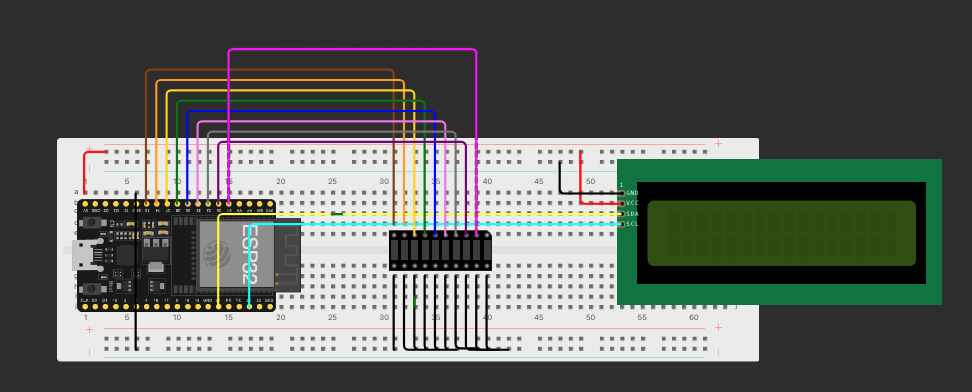
\includegraphics[width=0.8\textwidth]{../images/activity_monitor_scheme.png}
    \caption{Ultrasonic sensors connected to ESP01 modules.}
    \label{fig:esp32_system_monitor}
\end{figure}

\subsubsection{Data Flow and Configuration}

\subsection{MQTT Tree Structure}
The MQTT protocol in the presence and location project uses a structured approach to manage the data flow. Below is the outline of the MQTT topics and their functions:

\subsubsection{MQTT Topics}
\begin{itemize}
    \item \textbf{sensor1/distance:} This topic is used by the first ESP-01 module. It publishes the distance data measured by its connected ultrasonic sensor.
    \item \textbf{sensor2/distance:} Similar to the first, this topic is for the second ESP-01 module.
\end{itemize}

\subsubsection{Data Organization and Utilization}
The data sent to these topics include numerical values representing the measured distances. 

\end{document}

\end{document}